\documentclass[a4paper,11pt,oneside]{article}
% Add packages
\usepackage{graphics}	%NY
\usepackage{pifont}		%Symboler
\usepackage{afterpage}

\usepackage[T1]{fontenc}
\usepackage[utf8]{inputenc}
\usepackage[english,danish]{babel}
\usepackage{graphicx}
\usepackage{microtype}
\usepackage{lmodern}
\usepackage{lipsum}
\usepackage{makeidx} % Indexing package
\usepackage[intoc]{nomencl} % Nomenclature package
\usepackage{color}
\usepackage{mathpazo}
\usepackage[crop=pdfcrop]{pstool}
\usepackage{multirow}
\usepackage{textcomp}
%\usepackage[version=3]{mhchem}
\usepackage{relsize}
\usepackage{hyperref}
\usepackage{textpos}
\usepackage{indentfirst}
\usepackage{listings}
\usepackage{siunitx}
\usepackage{tikz}
\usetikzlibrary{shapes.geometric, arrows}
\usepackage[a4paper,left=3cm,right=3cm,top=3cm,bottom=3cm]{geometry}
\usepackage{wrapfig}
\usepackage{booktabs}
\usepackage{setspace}
\usepackage{mathptmx}
\usepackage{lmodern}
\usepackage{txfonts}
\usepackage{titlesec}
	\setcounter{secnumdepth}{4}

%\addto\captionsenglish{\renewcommand{\refname}{Litteraturliste}}
%\renewcommand{\bibname}{Litteraturliste}

\onehalfspacing

\setlength{\parindent}{1em}

\graphicspath{{pictures/}}

\everymath{\displaystyle}

% Avoid a warning
\pdfminorversion=5

\EndPreamble

%\usepackage{natbib} % Bibliography package
%\usepackage{siunitx} % Should stay after \EndPreamble

% Create a theorem environment
%\usepackage{amsthm}
\newtheorem{theorem}{Theorem}

\usepackage{xcolor,calc}

% Enable indexing
\makeindex

% Enable nomenclature
\makenomenclature

% Enable line numbering
%\usepackage{lineno}
%\pagewiselinenumbers
%\modulolinenumbers[5]

% Change table of contents name
\renewcommand*{\contentsname}{Table of Contents}

% Get a signature command
\makeatletter
\newcommand*{\getlength}[1]{\strip@pt#1}
\makeatother

\newlength{\signlength}
\setlength{\signlength}{0.5\textwidth}

\newcommand{\signature}[1]{%
\noindent \line(1,0){\getlength{\signlength}}\\
\noindent #1
}

% Add measuring units to nomenclature
\newcommand{\nomunit}[1]{\renewcommand{\nomentryend}{\hspace*{\fill}#1}}
\setlength{\belowcaptionskip}{10pt plus 5pt minus 5pt}

% Company logo
\def\bCompanyLogo{false}

% A fix for memoir-kluwer
\renewcommand{\bf}{\textbf}

% Set listings
\renewcommand\lstlistingname{Code snippet}
\renewcommand\lstlistlistingname{Code snippet}

\definecolor{white}{gray}{1.0}
\definecolor{light-gray}{gray}{0.95}
\definecolor{dkgreen}{rgb}{0,0.6,0}
\definecolor{gray}{rgb}{0.5,0.5,0.5}
\definecolor{mauve}{rgb}{0.58,0,0.82}

\lstset{
  frame=tb,
  language=C++,
  aboveskip=3mm,
  belowskip=3mm,
  showstringspaces=false,
  columns=flexible,
  basicstyle={\ttfamily},
  numbers=left,
  numberstyle=\tiny\color{gray},
  numbersep=11pt,                  
  stepnumber=1,                  
  captionpos = b,
  keywordstyle=\color{blue},
  commentstyle=\color{dkgreen},
  stringstyle=\color{mauve},
  backgroundcolor=\color{white},  
  breaklines=true,
  breakatwhitespace=true,
  tabsize=3,
  showspaces=false,
  showtabs=false
}



%Other setups

\usepackage{todonotes}
\graphicspath{{./pictures/}}
%\usepackage{amsmath}

\hypersetup{
    colorlinks,
    citecolor=green,
    filecolor=magenta,
    linkcolor=blue,
    urlcolor=cyan
}\hypersetup{
					colorlinks, 
					linkcolor={black},
					citecolor={blue!50!black},
					urlcolor={blue!80!black},
					}
\usepackage{fancyhdr}
\usepackage{lastpage}
\pagestyle{fancy}
\renewcommand{\sectionmark}[1]{\markright{\thesection.\ #1}}
\lhead{\korttitel}
\chead{}
\rhead{\rightmark}
\lfoot{\forfattere}
\cfoot{}
\rfoot{	\hfill \break
		\hfill \break
		Side \thepage \thinspace af \pageref{LastPage} \textbf{}}
\renewcommand{\headrulewidth}{0.5pt}
\renewcommand{\footrulewidth}{0.5pt}

\newcommand{\myparagraph}[1]{\paragraph{#1}\mbox{}\par}

\newcommand{\korttitel}{Tin Can Skype}
\newcommand{\forfattere}{
Anders Ellinge, 
Anders Fredensborg Rasmussen,
Daniel Holst Hviid,
Mathias Elbæk Gregersen
	\newline
Rasmus Skjerning Nielsen,
René Tidemand Haagensen,
Sarah Darmer Rasmussen
}

\usepackage{url}
\usepackage{hyperref}

\usepackage{comment}

%\usepackage[
%backend=biber,
%style=alphabetic,
%sorting=ynt
%]{biblatex}
%\addbibresource{ref.bib}

\begin{document}
	\definecolor{ColorH1}{rgb}{0.212,0.373,0.569}
\definecolor{ColorH2}{rgb}{0.141,0.197,0.376}
\definecolor{ColorH234}{rgb}{0.310,0.506,0.741}
\definecolor{ColorOthers}{rgb}{0.141,0.247,0.376}
\definecolor{White}{rgb}{1, 1, 1}
\definecolor{Gray}{rgb}{0.5, 0.5, 0.5}

\thispagestyle{empty}

\begin{center}        % Centrerer teksten
  \Huge
  \color{ColorH2}
  \textbf{\textit{Tin Can Skype}} 					\\
  \huge
  \textbf{\textit{RB-MRO3 - Gruppe 3}} 				\\
  \vspace{10mm}
  \color{Gray}
  \normalsize
  \bfseries{Uddannelse og semester:} 				\\
  \Large
  \color{ColorOthers}
  \normalfont{\textit{Robotteknologi - 3. semester}}\\
  \vspace{6mm}
  \color{Gray}
  \normalsize
  \bfseries{Afleveringsdato:} 						\\
  \Large
  \color{ColorOthers}
  \normalfont{\textit{18. December 2015}} 			\\
  \vspace{6mm}
  \color{Gray}
  \normalsize
  \bfseries{Vejleder:} 								\\
  \Large
  \color{ColorOthers}
  \normalfont{\textit{Ib Refer (refer@mmmi.sdu.dk)}}\\
  \vspace{6mm}
  \color{Gray}
  \normalsize
  \bfseries{Gruppemedlemmer:} 						\\
  \Large
  \color{ColorOthers}
  \normalfont{\textit{
 Anders Ellinge (aelli14@student.sdu.dk) 					\\ 
 Anders Fredensborg Rasmussen (andra14@student.sdu.dk) 		\\
 Daniel Holst Hviid (dahvi14@student.sdu.dk) 				\\
 Mathias Elbæk Gregersen (magre14@student.sdu.dk) 			\\
 Rasmus Skjerning Nielsen (rasni14@student.sdu.dk) 			\\
 René Tidemand Haagensen (rehaa14@student.sdu.dk) 			\\
 Sarah Darmer Rasmussen (srasm14@student.sdu.dk)
  }} \\
  \vspace{12mm}
  \begin{figure}[ht]
	\centering
	
\includegraphics[scale=0.25]{pictures/svg2.pdf} 
  \end{figure}
  \vspace{8mm}
  \normalsize
  \textsl{Det Tekniske Fakultet} 					\\
  \textsl{Syddansk Universitet} 					\\   
\end{center}
	\setcounter{page}{1}
	\pagenumbering{arabic}
	
	\section{Abstract}
This project demonstrates how to create at chat application using C++. The computers using the application must be able to communicate with DTMF tones and a communication protocol must be dessigned.
The created application also includes a login and user history feature.
\newline
Agile software development, in partucular Scrum, has been used to simplify our project challenges by dividing them into smaller issues.
\newline
The created software is divided into layered softwarearchitecture by using datacommunication layers, such as the physical layer, the data link layer, the transportation layer and the application layer. Our main issues were solved by using: Goertzel for efficient tone recognition, CRC for error detection in data packages and Stop-and-Wait for establishing a connection between two processes.
	\pagebreak
	\section{Forord}
Denne rapport er udarbejdet af gruppe 3, på andet semester på Civilingenør i Robotteknologi på Syddansk Universitet.
Rapporten er blevet skrevet i forbindelse med dette semesters projekt og beskriver hvordan denne gruppe har valgt at løse opgaverne i det valgte projekt, "Tin Can Skype", som er et chatprogram, der bruger DTMF-toner og indeholder bla. et simpelt log-in og historik system. 
\newline
Formålet med denne rapport er, at læseren skal være i stand til at læse og forstå projektet ved blot at have grundlæggende viden om C++ og datakommunikation, og ved at læse rapporten. 
\newline
\par
I forbindelse med dette projekt, blev følgende udstyr stillet til rådighed:
\begin{itemize}
	\item To mikrofoner
	\item To højtalere
\end{itemize}


	\pagebreak
	
	\tableofcontents
	\pagebreak
	
	
	\section{Indledning}
\subsection{Projektbeskrivelse}
I dette projekt er to højtalere og to mikrofoner blevet stillet til rådighed. Formålet med dette projekt er, at kunne sende data vha. DTMF-toner.
\newline
Det valgte projekt er et chatprogram, der udvikles i C++, og skal have de primære funktioner:
\begin{itemize}
	\item Overførsel af tekst.
	\item Log-in funktioner.
	\item Historik af chat-samtale.
\end{itemize}

Desuden er disse sekundære funktioner blevet overvejet:
\begin{itemize}
	\item Filoverførsel
	\item Gruppe chat
	\item Spil
	\item Redigering af tidligere beskeder
	\item Video streamings funktioner
	\item Humørikoner
\end{itemize}

Herudover er der desuden blevet overvejet at bruge en tredje computer, som kan bruges som en server.
Her vil mindst to computere altså være i stand til at kommunikere med hinanden vha. DTMF-toner.

\subsubsection{Krav til produktet}
Følgende krav blev stillet til projektet:
\begin{itemize}
	\item Bærbare computere skal kommunikere med hinanden, eller evt. et embedded system, ved	udveksling af lyd
	\item Der skal anvendes DTMF toner, og der skal designes en kommunikationsprotokol
	\item Der skal udvikles en distribueret applikation i C++
	\item Der skal anvendes en lagdelt softwarearkitektur
	\item Arkitekturen kunne være client/server med f.eks. tykke klienter
\end{itemize}
For at fuldføre dette projekt skal der anvendes to computere som skal være i stand til at kommunikere med hinanden ved hjælp af lyd i form af DTMF-toner. Derudover skal dette programmers i C++, her bruges klasser.

\subsubsection{Metodebeskrivelse}
Vi har i dette projekt valgt at benytte SCRUM, da alle gruppe medlemmer således er i stand til at arbejde med den metode der passer dem bedst. 
Vi har valgt at bruge brainstorm, som vores primære form for idégenererings-teknik.
Desuden prøver gruppen så vidt muligt at beregne alle de ting, der kan beregnes på forhånd.

\subsubsection{Afgrænsning}
Her ses de emner, som gruppen har overvejet at arbejde med. De primære funktioner er de funktioner som skal løses først, mens de sekundære løses efter tidsbegrænsning.
\newline
%Følgende punkter kan godt slettes hvis nødvendigt:
Primære funktioner:
\begin{itemize}
	\item Overførsel af tekst
		\subitem Protokol
		\subitem Karakter definition
		\subitem Størrelse
	\item Historik
		\subitem Tidspunkt
		\subitem Størrelse
	\item Log-in
\end{itemize}

Sekundære funktioner:
\begin{itemize}
	\item Fil-overførsel
		\subitem Protokol
		\subitem Queue
	\item Gruppe chat
		\subitem Protokol
	\item Spil database
		\subitem Protokol
		\subitem Funktion
	\item Rediger tidligere beskeder
		\subitem Protokol
		\subitem Funktion
	\item Stream funktion
		\subitem Protokol
		\subitem Funktion
	\item Humørikoner
		\subitem Char def.
		\subitem Database
	\item GUI
		\subitem Agil
	\item Sky "server"
		\subitem Funktion
\end{itemize}
	\subsection{Workload (product backlog)}
Der laves en product backlog i stedet for en tidplan (se figur \ref{fig:workload}).
\begin{figure}[ht]
	\centering
	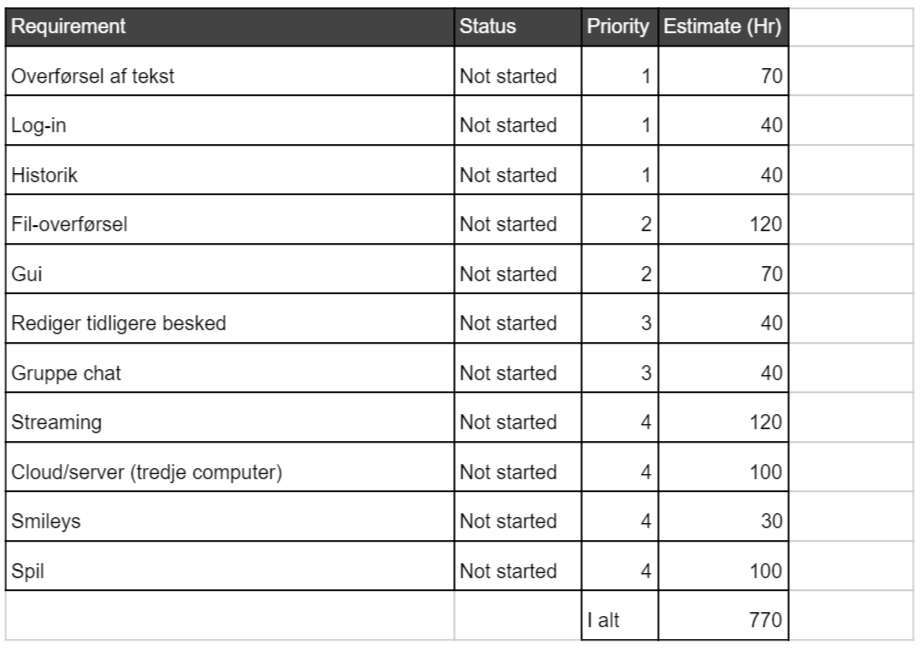
\includegraphics[width=15cm,height=25cm,keepaspectratio]{pictures/Workload.png}
	\caption{Product backlog}
	\label{fig:workload}
	\end{figure}
\newline
En product backlog er et værktøj inden for metoden SCRUM, som viser hvor langt tid en opgaver tager i mandetimer og hvilken status opgaven har (Not started, In process og Finished).

	\
%	\pagebreak
%	\input{sections/Random}
%	\pagebreak
%	\input{sections/Whatevs}
	\pagebreak
	\section{Konklusion}
Vi har ben
	\pagebreak
	\section{Perspektivering}
	\pagebreak
	
%	\section{Litteraturliste}
\begingroup
\renewcommand{\section}[2]{}%

\begin{thebibliography}{1}
	\subsection{Bøger}
  \bibitem{notes} John W. Dower {\em Readings compiled for History
  21.479.}  1991.

  \bibitem{impj}  The Japan Reader {\em Imperial Japan 1800-1945} 1973:
  Random House, N.Y.
  
	\subsection{Hjemmesider}
  \bibitem{norman} E. H. Norman {\em Japan's emergence as a modern
  state} 1940: International Secretariat, Institute of Pacific
  Relations.

  \bibitem{fo} Bob Tadashi Wakabayashi {\em Anti-Foreignism and Western
  Learning in Early-Modern Japan} 1986: Harvard University Press.

  \end{thebibliography}
	%\medskip
	%\printbibliography[title={Whole bibliography}]
	\section{Section}
	Ekstra stuff if needed
	
\end{document}